%% main.tex
%% Copyright 2022 Tom M. Ragonneau and Zaikun Zhang
%
% This work may be distributed and/or modified under the
% conditions of the LaTeX Project Public License, either version 1.3
% of this license or (at your option) any later version.
% The latest version of this license is in
%   http://www.latex-project.org/lppl.txt
% and version 1.3 or later is part of all distributions of LaTeX
% version 2005/12/01 or later.
%
% This work has the LPPL maintenance status `maintained'.
%
% The Current Maintainer of this work is Tom M. Ragonneau.
\documentclass[11pt,draft]{article}
\usepackage[T1]{fontenc}
\usepackage[american]{babel}
\usepackage[a4paper]{geometry}
\usepackage[final]{microtype}
\usepackage{csquotes}
\usepackage{lmodern}
\usepackage{booktabs}
\usepackage{siunitx}

% Graphics and captions
\usepackage{graphicx}
\usepackage[tableposition=top]{caption}
\usepackage{subcaption}
\graphicspath{{images/}}

% Bibliography information processing
\usepackage[
    style=numeric-comp,
    sorting=nyt,
    sortcites=false,
]{biblatex}
\addbibresource{ragonneau-bib/strings.bib}
\addbibresource{ragonneau-bib/optim.bib}

% Terms and acronyms processing
\usepackage[acronym]{glossaries-extra}
\glsdisablehyper
\newabbreviation{auc}{AUC}{area under the curve}
\newabbreviation{dfo}{DFO}{derivative-free optimization}
\newabbreviation{kkt}{KKT}{Karush-Kuhn-Tucker}
\newabbreviation{rbf}{RBF}{radial basis function}
\newabbreviation{roc}{ROC}{receiver operating characteristic}
\newabbreviation{rs}{RS}{random search}
\newabbreviation{svm}{SVM}{support vector machine}
\newabbreviation{tpe}{TPE}{tree of Parzen estimators}
\newacronym{bobyqa}{BOBYQA}{Bound Optimization BY Quadratic Approximation}
\newacronym{cobyla}{COBYLA}{Constrained Optimization BY Linear Approximations}
\newacronym{lincoa}{LINCOA}{LINearly Constrained Optimization Algorithm}
\newacronym{newuoa}{NEWUOA}{NEW Unconstrained Optimization Algorithm}
\newacronym{uobyqa}{UOBYQA}{Unconstrained Optimization BY Quadratic Approximation}
\newacronym{pdfo}{PDFO}{Powell's derivative-free optimization solvers}

% Mathematical expressions
\usepackage{amsmath}
\usepackage{amsfonts}
\usepackage{amssymb}
\usepackage{dsfont}
\usepackage{xargs}
\numberwithin{equation}{section}

\DeclareMathOperator*\argmin{arg\,min}
\DeclareMathOperator\rank{rank}
\DeclareMathOperator\range{\mathcal{R}}

\def\defeq{\ensuremath{\mathrel{\stackrel{\text{\tiny\textsf{def}}}{=}}}}
\def\sft{\ensuremath{\mathsf{T}}}
\def\R{\ensuremath{\mathbb{R}}}
\newcommand\abs[2][]{#1|#2#1|}
\newcommand\norm[2][]{#1\|#2#1\|}
\newcommand\set[2][]{#1\{#2#1\}}
\def\obj{\ensuremath{f}}
\def\srchsp{\ensuremath{\Omega}}
\def\bl{\ensuremath{l}}
\def\bu{\ensuremath{u}}
\newcommand\cgen[1][i]{c_{#1}}
\def\ceq{\ensuremath{\cgen[\scriptscriptstyle\mathcal{E}]}}
\def\cub{\ensuremath{\cgen[\scriptscriptstyle\mathcal{I}]}}
\def\aeq{\ensuremath{A_{\scriptscriptstyle\mathcal{E}}}}
\def\beq{\ensuremath{b_{\scriptscriptstyle\mathcal{E}}}}
\def\aub{\ensuremath{A_{\scriptscriptstyle\mathcal{I}}}}
\def\bub{\ensuremath{b_{\scriptscriptstyle\mathcal{I}}}}
\newcommand\objmdl[1][k]{\obj_{#1}}
\newcommand\srchspmdl[1][k]{\Omega_{#1}}
\newcommandx\cgenmdl[2][1=k,2=i]{c_{#2,#1}}
\newcommand\iter[1][k]{x_{#1}}
\newcommand\trg[1][k]{\Delta_{#1}}
\newcommand\itpls[1][k]{\mathcal{Y}_{#1}}
\newcommand\grad[1][k]{g_{#1}}
\newcommand\hess[1][k]{B_{#1}}
\newcommand\trial{{\text{t}}}
\newcommand\geo{{\text{g}}}

% Cross-referencing and colorization
% Note: hyperref must be imported after amsmath.
\usepackage[final,hyperfootnotes=false]{hyperref}
\usepackage[dvipsnames]{xcolor}
\usepackage{url}
\hypersetup{
    colorlinks=true,
    linkcolor=OliveGreen,
    anchorcolor=black,
    citecolor=MidnightBlue,
    filecolor=black,
    menucolor=black,
    runcolor=black,
    urlcolor=black,
}

% Automatic references
% Note: cleveref must be imported after hyperref.
\usepackage[noabbrev]{cleveref}
\crefname{equation}{}{}
\Crefname{equation}{}{}
\crefname{lstlisting}{listing}{listings}
\Crefname{lstlisting}{Listing}{Listings}

% Customize list environments
\usepackage{enumitem}
\setitemize{
    topsep=\parsep,
    itemsep=0pt,
}
\setenumerate{
    topsep=\parsep,
    itemsep=0pt,
}

% Customize listings environments
\usepackage[final]{listings}
\usepackage{lstautogobble}
\lstset{
    autogobble=true,
    basicstyle=\normalsize\ttfamily,
    breakautoindent=true,
    breakatwhitespace=false,
    breaklines=true,
    commentstyle=\itshape\color{black!50},
    frame=tb,
    keywordstyle=\bfseries\color{MidnightBlue},
    numbers=left,
    numberstyle=\scriptsize\color{CadetBlue!75},
    postbreak=\space,
    showstringspaces=false,
    stepnumber=1,
    stringstyle=\color{OliveGreen},
    tabsize=4,
}
\lstnewenvironment{matlablst}[1][]{
    \lstset{
        language=matlab,
        morekeywords={ones},
        #1,
    }
}{}

% Spacing between lines
\linespread{1.1}

% List of hyphenation exceptions for US English
% Source: https://ctan.org/tex-archive/info/digests/tugboat/hyphenex
\input{ushyphex}

% General macros
\def\bfo{\mbox{BFO}}
\def\boosters{\mbox{BOOSTERS}}
\def\conorbit{\mbox{CONORBIT}}
\def\cutest{\mbox{CUTEst}}
\def\dfls{\mbox{DFLS}}
\def\dfols{\mbox{DFO-LS}}
\def\dfotr{\mbox{DFO-TR}}
\def\dfp{\mbox{DFP}}
\def\fortran{\mbox{Fortran}}
\def\julia{\mbox{Julia}}
\def\libsvm{\mbox{LIBSVM}}
\def\mads{\mbox{MADS}}
\def\matlab{\mbox{MATLAB\textsuperscript{\textregistered}}}
\def\matlabopt{\mbox{\matlab\ Optimization Toolbox\textsuperscript{\texttrademark}}}
\def\minqa{\mbox{\texttt{minqa}}}
\def\mnh{\mbox{MNH}}
\def\nlopt{\mbox{NLopt}}
\def\orbit{\mbox{ORBIT}}
\def\pybobyqa{\mbox{Py-BOBYQA}}
\def\python{\mbox{Python}}
\def\rlang{\mbox{R}}
\def\scipy{\mbox{SciPy}}
\def\sklearn{\mbox{scikit-learn}}

% Drafting macros
\usepackage{ifdraft}
\usepackage[
    obeyDraft,
    backgroundcolor=BurntOrange,
    textsize=scriptsize,
]{todonotes}
\ifdraft{
    \usepackage{draftwatermark}
    \usepackage{refcheck}
    \SetWatermarkColor{Gray}
    \SetWatermarkLightness{0.9}
}{}

% Article metadata
\usepackage{titling}
\title{PDFO --- Cross-Platform Package for Using Powell's Derivative-Free Optimization Solvers}
\author{
    Tom M. Ragonneau\thanks{
        Department of Applied Mathematics,
        The Hong Kong Polytechnic University,
        Hung Hom, Kowloon, Hong Kong
        (\href{mailto:tom.ragonneau@connect.polyu.hk}{\texttt{tom.ragonneau@connect.polyu.hk}}).
        Support for this author was provided by the University Grants Committee of Hong Kong under the Hong Kong Ph.D. Fellowship Scheme (ref.\ PF18-24698).
    }
    \and Zaikun Zhang\thanks{
        Department of Applied Mathematics,
        The Hong Kong Polytechnic University,
        Hung Hom, Kowloon, Hong Kong
        (\href{mailto:zaikun.zhang@polyu.edu.hk}{\texttt{zaikun.zhang@polyu.edu.hk}}).
        Support for this author was partially provided by the University Grants Committee of Hong Kong under the  Early Career Scheme (ref.\ PolyU 253012/17P and PolyU 153054/20P) and The Hong Kong Polytechnic University (ref.\ P0009767).
    }
}
\date{\today}
\hypersetup{
    pdftitle=\thetitle,
    pdfauthor=\texorpdfstring{\theauthor}{Tom M. Ragonneau and Zaikun Zhang},
    pdfsubject={},
    pdfkeywords={},
}

\begin{document}

\maketitle

\begin{abstract}
    To do.
\end{abstract}

\section{Introduction}

Most optimization algorithms rely on classical or generalized derivative information of the objective function and constraints.
However, in many applications, such information is not available.
This is the case, for example, if the objective function does not have an explicit formulation but can only be evaluated through complex simulations or experiments.
Optimization problems of such kind arise from automatic error analysis~\cite{Higham_1993,Higham_2002}, machine learning~\cite{Ghanbari_Scheinberg_2017}, analog circuit design~\cite{Latorre_Etal_2019}, aircraft engineering~\cite{Gazaix_Etal_2019}, and chemical product design~\cite{Sun_Etal_2020}, to name but a few.
These problems motivate the development of optimization algorithms that use only function values but not derivatives.

Between~\citeyear{Powell_1994} and~\citeyear{Powell_2015}, Powell developed five solvers to tackle unconstrained and constrained problems without using derivatives,
namely~\gls{cobyla}~\cite{Powell_1994}, \gls{uobyqa}~\cite{Powell_2002}, \gls{newuoa}~\cite{Powell_2006}, \gls{bobyqa}~\cite{Powell_2009}, and \gls{lincoa}.
These solvers were implemented by Powell, with particular attention paid to their numerical stability and algebraic complexity.
Renowned for their robustness and efficiency, these solvers are extremely appealing to practitioners and widely used in applications, for instance, aeronautical engineering~\cite{Gallard_Etal_2018b}, astronomy~\cite{Biviano_Etal_2013,Mamon_Biviano_Boue_2013}, computer vision~\cite{Izadinia_Shan_Seitz_2017}, robotics~\cite{Mombaur_Truong_Laumond_2010}, and statistics~\cite{Bates_Etal_2015}.

However, Powell coded in \fortran\ 77, an old-fashion language that damps the enthusiasm of many users to exploit these solvers in their projects.
There have been a considerable demand from both researchers and practitioners for the availability of Powell's solvers in more user-friendly languages such as \python, \matlab, and \julia.
Our aim is to wrap Powell's \fortran\ code into a package named~\gls{pdfo}, which enables users of such languages to call Powell's solvers without any need of dealing with the \fortran\ code.
For each supported language, \gls{pdfo} provides a simple subroutine that can invoke one of Powell's solvers according to the user's request (if any) or according to the type of the problem to solve. The current release (version 1.1) of \gls{pdfo} supports \python\ and \matlab, with more languages to be covered in the future.
The signature of the \python\ subroutine is consistent with the \texttt{minimize} function of the \scipy\ optimization library;
the signature of the \matlab\ subroutine is consistent with the \texttt{fmincon} function of the \matlabopt.
The package is cross-platform, available on Linux, macOS, and Microsoft Windows at once.

\gls{pdfo} is not the first attempt to facilitate the usage of Powell's solvers in languages other than \fortran.
Various efforts have been made in this direction in response to the continual demands from both researchers and practitioners: \pybobyqa~\cite{Cartis_Etal_2019} provides a \python\ implementation of \gls{bobyqa}; \nlopt~\cite{Johnson_2019} includes multi-language interfaces for \gls{cobyla}, \gls{newuoa}, and \gls{bobyqa}; \minqa~\cite{Bates_Etal_2014} wraps \gls{uobyqa}, \gls{newuoa}, and \gls{bobyqa} in \rlang; \scipy~\cite{Virtanen_Etal_2020} makes \gls{cobyla} available in \python\ under its optimization library. Nevertheless, \gls{pdfo} has several features that distinguishes itself from others.

\begin{enumerate}
    \item \emph{Comprehensiveness.}
    To the best of our knowledge, \gls{pdfo} is the only package that provides all of \gls{cobyla}, \gls{uobyqa}, \gls{newuoa}, \gls{bobyqa}, and \gls{lincoa} with a uniform interface.
    In addition to homogenizing the usage, such an interface eases the comparison between these solvers in case multiple of them are able to tackle a given problem.
    Doing so, we may gain insights that cannot be obtained otherwise into the behavior of the solvers, as will be illustrated in~\cref{sec:fake}.

    \item \emph{Solver selection.}
    When using \gls{pdfo}, the user can specifically call one of Powell's solvers; nevertheless, if the user does not specify any solver, \gls{pdfo} will select automatically a solver according to the given problem.
    The selection takes into consideration the performance of the solvers on the \cutest~\cite{Gould_Orban_Toint_2015} problem set.
    Interestingly, it turns out that the solver with the best performance may not be the most intuitive one.
    For example, \gls{newuoa} is not always the best choice for solving an unconstrained problem.
    This will be elaborated in~\cref{sec:fake}

    \item \emph{Code patching.}
    During the development of \gls{pdfo}, we spotted in the original \fortran\ code some bugs, which led to infinite cycling or segmentation faults on some ill-conditioned problems.
    The bugs have been patched in \gls{pdfo}.
    Nevertheless, we provide an option that can enforce the package to use the original code of Powell without the patches, which is not recommended except for research.
    In addition, \gls{pdfo} provides \gls{cobyla} in double precision, whereas Powell used single precision when he implemented it in the 1990s. See~\cref{sec:fake} for details.

    \item \emph{Fault tolerance.}
    \gls{pdfo} takes care of failures in the evaluation of the objective or constraint functions when NaN or infinite values are returned.
    In case of such failures, \gls{pdfo} will not exit but try to progress.
    Moreover, \gls{pdfo} ensures that the returned solution is not a point where the evaluation fails, while the original code of Powell may return a point whose objective function value is numerically NaN. This is explained in~\cref{sec:fake}.

    \item \emph{Problem preprocessing.}
    \gls{pdfo} preprocesses the inputs to simplify the problem and reformulate it to meet the requirements of Powell's solvers.
    For instance, if the problem has linear constraints~$A x = b$, \gls{pdfo} can rewrite it into a problem on the null space of~$A$, eliminating such constraints and reducing the dimension.
    Another example is that the starting point of a linearly-constrained problem is projected to the feasible region, because \gls{lincoa} needs a feasible starting point to work properly.

    \item \emph{Additional options.}
    \gls{pdfo} includes options for the user to control the solvers in some manners that are useful in practice.
    For example, the user can request \gls{pdfo} to scale the problem according to the bounds of the variables before solving it.

\end{enumerate}

The organization of this paper is as follows: \cref{sec:powell} presents a brief description of the five Powell's \gls{dfo} algorithms and \cref{sec:pdfo} introduces \gls{pdfo}, a cross-platform package providing \matlab\ and \python\ interfaces for using the above-mentioned solvers.

\section{A brief review of \texorpdfstring{\glsfmtshort{dfo}}{DFO methods}}

Consider a nonlinear optimization problem
\begin{equation}
    \label{eq:nlc}
    \min_{x \in \srchsp} \obj(x),
\end{equation}
where~$\obj \colon \R^n \to \R$ is the objective function and~$\srchsp \subseteq \R^n$ refers to the feasible region of the problem.
As summarized in~\cite{Conn_Scheinberg_Vicente_2009b}, two strategies have been developed to tackle the problem~\cref{eq:nlc} without using derivatives, which we will sketch in the sequel.

The first strategy, known as direct search,\footnote{\,In some early papers (e.g., \cite{Powell_1994,Powell_1998}), Powell used \enquote{direct search} to mean what is known as \enquote{derivative-free optimization} today.} explores the objective function~$\obj$ and chooses iterates by simple comparisons of function values, examples including the Nelder-Mead algorithm~\cite{Nelder_Mead_1965}, the \mads\ methods~\cite{Audet_Dennis_2006,Abramson_Audet_2006,Digabel_2011}, and \bfo~\cite{Porcelli_Toint_2017,Porcelli_Toint_2020,Porcelli_Toint_2021}.
See~\cite{Kolda_Lewis_Torczon_2003},~\cite[Chapters~7 and~8]{Conn_Scheinberg_Vicente_2009b},~\cite[Part~3]{Audet_Hare_2017}, and~\cite[Section~2.1]{Larson_Menickelly_Wild_2019} for more discussions on this paradigm, and we refer to~\cite{Gratton_Etal_2015,Gratton_Etal_2019} for recent developments on randomized methods in this category.

The second strategy approximates the original problem~\cref{eq:nlc} by relatively simple models and locates the iterates according to such models.
Algorithms with this strategy are referred to as model-based methods, and they often make use of the
models within a trust-region framework~\cite{Conn_Gould_Toint_2000,Conn_Scheinberg_Vicente_2009a,Yuan_2015}, but line search methods also exist~\cite{Berahas_Byrd_Nocedal_2019,Shi_Etal_2021}.
Interpolation and regression are two common ways of establishing the models~\cite{Powell_2001,Powell_2004a,Conn_Scheinberg_Vicente_2008a,Conn_Scheinberg_Vicente_2008a,Wild_Regis_Shoemaker_2008,Bandeira_Scheinberg_Vicente_2012,Billups_Larson_Graf_2013,Regis_Wild_2017}.
Algorithms using finite-difference approximations of gradients can also be regarded as model-based methods, because such approximations essentially come from linear (for forward and backward finite differences) or quadratic (for central finite difference) interpolation of the function under consideration over rather special interpolation sets.
Most model-based \gls{dfo} methods employ polynomial models that are linear or quadratic, examples including
Powell's methods~\cite{Powell_1994,Powell_2002,Powell_2006,Powell_2009}, \mnh~\cite{Wild_2008}, \dfls~\cite{Zhang_Conn_Scheinberg_2010}, \dfotr~\cite{Bandeira_Scheinberg_Vicente_2012}, and \dfols~\cite{Cartis_Etal_2019}, but there are also successful cases exploiting~\glspl{rbf},
such as \orbit~\cite{Wild_Regis_Shoemaker_2008}, \conorbit~\cite{Regis_Wild_2017}, and \boosters~\cite{Oeuvray_Bierlaire_2009}.
Model-based \gls{dfo} is one of the motivations for studying trust-region and line search methods with
randomized models, for which we refer to~\cite{Bandeira_Scheinberg_Vicente_2014,Gratton_Etal_2018,Cartis_Scheinberg_2018} as examples.

Hybrids between direct search and model-based approaches exist, for example~\cite{Custodio_Vicente_2007}, \cite[Algorithm~4.7]{Kelley_2011}, and~\cite{Conn_Digabel_2013}.
Theory of global convergence and convergence rate has been established for both direct search and model-based methods~\cite{Torczon_1997,Conn_Scheinberg_Toint_1997a,Kolda_Lewis_Torczon_2003,Conn_Scheinberg_Vicente_2009a,Powell_2012,Vicente_2013,Dodangeh_Vicente_2016,Garmanjani_Judice_Vicente_2016,Gratton_Royer_Vicente_2020}.
It is worth noting that the performance of \gls{dfo} algorithms are measured in general by the number of function evaluations needed for solving a given problem, because the objective and constraint functions in \gls{dfo} problems are commonly expensive to evaluate.
Therefore, the worst-case complexity in terms of function evaluations is a major theoretical aspect of~\gls{dfo} algorithms.
Examples of such complexity analysis can be found in~\cite{Vicente_2013,Gratton_Etal_2015,Dodangeh_Vicente_2016,Dodangeh_Vicente_Zhang_2016}.
For more extensive discussions on \gls{dfo} methods and theory, see the monographs~\cite{Conn_Scheinberg_Vicente_2009b,Audet_Hare_2017}, the survey papers~\cite{Rios_Sahinidis_2013,Custodio_Scheinberg_Vicente_2017,Larson_Menickelly_Wild_2019}, and the references therein.

\section{Powell's derivative-free methods}
\label{sec:powell}

Powell published his first \gls{dfo} algorithm based on conjugate directions in \citeyear{Powell_1964}~\cite{Powell_1964}\footnote{\,According to Google Scholar, this is Powell's second published paper and also the second most cited work.
The earliest and meanwhile most cited one is his paper on the \dfp\ method~\cite{Fletcher_Powell_1963}, co-authored with Fletcher and published in 1963.}.
His code for this algorithm is contained in the HSL Mathematical Software Library~\cite{HSL} as subroutine \texttt{VA24}.
It is not included in \gls{pdfo} because the code is not in the public domain, although open-source implementations are available~(see~\cite[footnote~4]{Conn_Scheinberg_Toint_1997b}).

From the 1990s to the final days of his career, Powell developed five model-based \gls{dfo} algorithms to solve~\cref{eq:nlc}, namely \gls{cobyla}~\cite{Powell_1994}~(for nonlinearly-constrained problems), \gls{uobyqa}~\cite{Powell_2002}~(for unconstrained problems), \gls{newuoa}~\cite{Powell_2006}~(for unconstrained problems), \gls{bobyqa}~\cite{Powell_2009}~(for bound-constrained problems), and~\gls{lincoa} (for linearly constrained problems).
In addition, Powell implemented these algorithms into \fortran~solvers and made the code publicly available.
The solvers constitute the cornerstone of~\gls{pdfo}.
In the sequel, we provide a brief overview on these five algorithms.

Powell's model-based \gls{dfo} algorithms are trust-region methods with linear or quadratic interpolation models.
At iteration~$k$, the algorithms maintain a finite set~$\itpls \subseteq \R^n$ of interpolation points, and construct a model~$\objmdl$ satisfying the interpolation conditions
\begin{equation}
    \label{eq:itpls}
    \objmdl(y) = \obj(y), \quad y \in \itpls.
\end{equation}
The trust region center~$\iter$ is a point chosen from~$\itpls$ according to the value of a merit function or the objective function.
A trial point~$\iter^{\trial}$ is then obtained by solving approximately
\begin{subequations}
    \label{eq:trsp}
    \begin{align}
        \min_{x \in \srchspmdl} & \quad \objmdl(x)\\
        \text{s.t.}             & \quad \norm{x - \iter} \le \trg, \label{eq:trsp-tr}
    \end{align}
\end{subequations}
where~$\trg$ is the trust-region radius,~$\norm{\cdot}$ is the~$2$-norm in~$\R^n$, and the feasible region~$\srchsp$ is modeled locally by a set~$\srchspmdl \subseteq \R^n$, which can be~$\srchsp$ itself.
The strategy to update~$\itpls$ is crucial.
It should recycle points from previous iterations, at which the objective function has already been evaluated; meanwhile, it needs to maintain the well poisedness~\cite{Sauer_Xu_1995,Conn_Scheinberg_Vicente_2009b} of the interpolation set in order to guarantee the accuracy of the interpolants.
\todo{The sentence seems incomplete.}After the
$$\itpls[k+1] = \itpls \cup \{\iter^{\trial}\} \setminus\{y_k^{\trial}\}$$
$$\itpls[k+1] = \itpls \setminus\{y_k^{\geo}\} \cup \{\iter^{\geo}\}$$
and ensure the convergence of the optimization algorithm~\cite{Conn_Scheinberg_Vicente_2008a,Conn_Scheinberg_Vicente_2008b,Fasano_Morales_Nocedal_2009,Scheinberg_Toint_2010}.

\subsection{\texorpdfstring{\glsfmtshort{cobyla}}{COBYLA}}

At the dawn of the modern \gls{dfo}, Powell introduced in \citedate{Powell_1994} his solver \gls{cobyla}~\cite{Powell_1994}, named after \enquote{\glsxtrlong{cobyla}}.
It attempts to solve the optimization problem~\cref{eq:nlc} when the feasible region~$\srchsp$ is general and expressed as
$$\srchsp \defeq \set{x \in \R^n \colon \cgen(x) \ge 0,\; i=1,...,m},$$
where~$\cgen \colon \R^n \to \R$ denotes the~$i$th nonlinear constraint function, with~$i \in \set{1, 2, \dots, m}$.
At each iteration, it approximates the objective and constraint functions with linear models obtained by fully-determined interpolations on~$\itpls$, whose cardinal is fixed to~$n + 1$.
In this context, the poisedness~\cite[\S 1]{Sauer_Xu_1995} of the interpolation set, i.e., the geometrical condition on~$\itpls$ required to ensure the uniqueness of the models, can be seen as the volume of the~$n$-simplex engendered by~$\itpls$ to be nonzero.
Once the linear models~$\cgenmdl$ of the constraint functions~$\cgen$ for~$i \in \set{1, 2, \dots, m}$ are built, an approximation~$\srchspmdl$ of~$\srchsp$ is obtained as the intersection of the half-spaces generated by the linear approximations of the constraint functions, that is
\begin{equation}
    \label{eq:cobylarg}
    \srchspmdl \defeq \set{x \in \R^n \colon \cgenmdl(x) \ge 0,\; i=1,...,m},
\end{equation}
and the trust-region subproblem~\cref{eq:trsp} is then solved.
As a linear programming problem, the trust-region subproblem is solved in the following way.
Solving sequentially the problems~\cref{eq:trsp} by replacing the trust-region radius~$\trg$ by a constant continuously evolving from~$0$ to~$\trg$ would generate a continuous piecewise linear path from~$\iter$ to the solution of the subproblem.
The strategy of COBYLA is to compute this path, by updating the active sets of the constraint models.
However, the trust-region condition~\cref{eq:trsp-tr} and the region~\cref{eq:cobylarg} may contradict each others, in which case the trial point is chosen to solve approximately
\begin{align*}
    \max_{x \in \R^n}   & \quad \min_{i = 1, 2, \dots, m} \cgenmdl(x)\\
    \text{s.t.}         & \quad \norm{x - \iter} \le \trg.
\end{align*}
In doing so, the method attempts to reduce some violation of the constraint models while ensuring that the trial point lies in the trust region, as it is needed by most global convergence properties.

\subsection{\texorpdfstring{\glsfmtshort{uobyqa}}{UOBYQA}}

Later on, in \citedate{Powell_2002}, Powell developed \gls{uobyqa}~\cite{Powell_2002}, named after \enquote{\glsxtrlong{uobyqa}}.
It aims at solving the nonlinear optimization problem~\cref{eq:nlc} in the unconstrained case, i.e., when~$\srchsp = \R^n$.
To do so, at each iteration, it models the objective function with a quadratic of the form~\cref{eq:polm}, obtained by fully-determined interpolation on the set~$\itpls$ containing~$N = (n + 1)(n + 2) / 2$ points.
The set~$\itpls[k + 1]$ differs from~$\itpls$ of at most one point.
During a classical iteration, a trial point, i.e., an approximate solution of the trust-region subproblem~\cref{eq:trsp} replaces an interpolation of~$\itpls$.
As we already mentioned, it is essential to maintain some geometrical properties of~$\itpls$ to ensure the existence and the uniqueness of the models from a computational viewpoint.
Hence, \gls{uobyqa} may undertake geometry-improvement steps whenever the models seem not to be accurate, led a remarkable result pointed out in~\cite{Powell_2001}.
It states that given a point~$\bar{y} \in \itpls$ to remove from the interpolation set, its most suitable substitute to build~$\itpls[k + 1]$ solves the subproblem
\begin{equation}
    \label{eq:biglag}
    \begin{aligned}
        \max_{x \in \R^n}   & \quad \abs{\ell_{\bar{y}}(x)}\\
        \text{s.t.}         & \quad \norm{x - \iter} \le \trg,
    \end{aligned}
\end{equation}
where~$\ell_{\bar{y}} \colon \R^n \to \R$ denotes the Lagrange function associated with~$\bar{y}$, defined by~$\ell_{\bar{y}}(y) = \delta_{\bar{y}, y}$ for each~$y \in \itpls$, where~$\delta_{\bar{y}, y}$ is the Kronecker delta.
Since \gls{uobyqa} requires only a rough solution of the geometry-improvement subproblem~\cref{eq:biglag}, Powell developed an algorithm that requires only~$\mathcal{O}(n^2)$ operations, based on an estimation of~$\abs{\ell_{\bar{y}}(\cdot)}$.
Once such a point is calculated, the solver continues with a classical trust-region step, and the subproblem~\cref{eq:trsp} is solved with the Mor{\'{e}}-Sorensen algorithm~\cite{More_Sorensen_1983}, as it controls the accuracy of the solution.

\subsection{\texorpdfstring{\glsfmtshort{newuoa}}{NEWUOA}, \texorpdfstring{\glsfmtshort{bobyqa}}{BOBYQA}, and~\texorpdfstring{\glsfmtshort{lincoa}}{LINCOA}}

The major flaw of \gls{uobyqa} is the amount of required interpolation points, which can become prohibitively huge when~$n$ increases.
Therefore, Powell designed a mechanism to define quadratic models of the form~\cref{eq:polm} that requires fewer interpolation points~\cite{Powell_2004a}.
Given the set~$\itpls$, containing typically~$\mathcal{O}(n)$ points (the default value~$2n + 1$ being recommended), the model~$\objmdl$ is the quadratic satisfying the interpolation conditions whose Hessian's update is least in Frobenius norm, that is
\begin{equation}
    \label{eq:varmod}
    \begin{aligned}
        \objmdl \defeq \argmin_{Q \in \mathcal{P}_{n, 2}}   & \quad \norm{\nabla^2 Q - \nabla^2 \objmdl[k - 1]}_{\mathsf{F}}\\
        \text{s.t.}                                         & \quad Q(y) = \obj(y), \quad y \in \itpls,
    \end{aligned}
\end{equation}
where~$\mathcal{P}_{n, d}$ is the space of~$n$-variate polynomials of degree at most~$d$ and~$\nabla^2 \objmdl[-1]$ is set to be zero.
If the number of interpolation points was less than or equal to~$n + 1$, the models would remain linear, so that Powell requires the number of points in~$\itpls$ to be at least~$n + 2$ and at most~$(n + 1)(n + 2) / 2$.
As we mentioned earlier, the choice of the variational problem~\cref{eq:varmod} is fostered by the fact that it occurs in the quasi-Newton update for unconstrained optimization when the first derivative of the objective function is available~\cite[\S 3.6]{Fletcher_1987}.
As in the fully-determined case, the geometry of the interpolation set plays a crucial role, as it influences the accuracy of the quadratic models, and the geometry-improvement steps~\cref{eq:biglag} should be also entertained.

The last three \gls{dfo} solvers of Powell are \gls{newuoa}~\cite{Powell_2006, Powell_2008},
\gls{bobyqa}~\cite{Powell_2009}, and~\gls{lincoa}.
\Gls{bobyqa} and \gls{lincoa} are named respectively after \enquote{\glsxtrlong{bobyqa}} and \enquote{\glsxtrlong{lincoa}}, but the meaning of the acronym \gls{newuoa} is not known (even though most people agree on \enquote{\glsxtrlong{newuoa}}).
Powell never published a paper introducing \gls{lincoa}, and~\cite{Powell_2015} discusses only the resolution of its trust-region subproblem.
As their names suggest, they aim at solving unconstrained, bound-constrained and linearly-constrained problems respectively, using quadratic models of the objective function of the form~\cref{eq:polm}.
All three use the underdetermined interpolation technique described above to build the quadratic models, so that \gls{newuoa} is more suitable than \gls{uobyqa} for solving problems with a relatively high dimension.
They all set~$\srchspmdl$ in the trust-region subproblem~\cref{eq:trsp} to be~$\Omega$, corresponding the whole space for \gls{newuoa}, a box for \gls{bobyqa} and a polyhedron for \gls{lincoa}.
A subtlety of \gls{bobyqa} is that the constraints are always respected, for each iterate and each point in~$\itpls$.
Therefore, the geometry-improvement subproblem~\cref{eq:biglag} should be adapted to incorporate the bound constraints, which makes its resolution more difficult.
Moreover, as we already mentioned, at most one point of the interpolation set is altered at each iteration, which leads to an at-most rank-$2$ update of the \gls{kkt} matrix of the variational problem~\cref{eq:varmod}.
This remark suggests that it can be much more efficient to update such \gls{kkt} matrix instead of computing it from scratch at each iteration.
Powell derived an updating formula in~\cite{Powell_2004b} that requires only~$\mathcal{O}(N^2)$ operations instead of~$\mathcal{O}(N^3)$ if the computation was made from scratch with no loss of accuracy, where~$N$ denotes the number of interpolation points.
When it comes to solving the trust-region subproblems~\cref{eq:trsp}, \gls{newuoa} employs the Steihaug-Toint truncated conjugate gradient algorithm~\cite{Steihaug_1983, Toint_1981}, and \gls{bobyqa} and \gls{lincoa} use an active-set variation of it.
However, the trust-region subproblem solver of \gls{bobyqa} always respects the bounds, while the solver of \gls{lincoa} may visit point lying outside of the polyhedron of the constraints, and may even return points that are slightly infeasible.


\subsection{Geometry steps}

We focus however our attention on polynomial models of the form
\begin{equation}
    \label{eq:polm}
    \objmdl(x) \defeq \grad^{\sft} (x - \iter) + (x - \iter)^{\sft} \hess (x - \iter),
\end{equation}
with~$\grad \in \R^n$ and~$\hess \in \R^{n \times n}$ being symmetric and may be zero for linear models, diagonal or general depending on the considered method.
Such models admit respectively~$n + 1$,~$2n + 1$ and~$(n + 1)(n + 2) / 2$ coefficients, determined so that they satisfy the interpolation conditions~\cref{eq:itpls}.
Whenever the models are defined by underdetermined interpolations, the freedom bequeathed by the interpolation conditions is usually taken up by a variational problem whose constraints are the conditions~\cref{eq:itpls}.
Examples of such variational problems are the minimization of the Hessian of the models in Frobenius norm~\cite{Conn_Scheinberg_Toint_1998, Wild_2008}, or the minimization of a term involving~$\grad$ and~$\hess$ in~\cref{eq:polm}~\cite{Conn_Toint_1996}.
Powell employed another example of such variational problem, namely the symmetric Broyden formula~\cite{Powell_1970b, Powell_2004a}, which will be studied later in this paper in \cref{sec:powell}.

\section{An interface for the Powell's derivative-free solvers}
\label{sec:pdfo}

Powell implemented all five methods in \fortran, in a very robust and efficient manner.
However, less and less people are using \fortran\ in our present-day world, and \fortran\ has quite old standards.
The authors developed therefore \gls{pdfo}\footnote{Available at \url{https://www.pdfo.net/}.}, named after \enquote{\glsxtrlong{pdfo}}.
It is cross-platform package providing \matlab\ and \python\ interfaces for using all five Powell's \gls{dfo} solvers, available for Linux, macOS and Windows.
\Gls{pdfo} does not reimplement Powell's solvers, but rather links the modern languages \matlab\ and \python\ with the \fortran\ source code.
At a low-level, it uses F2PY~\cite{Peterson_2009} to interface \python\ with \fortran\, and MEX to interface it with \matlab.

\subsection{Main structure of the package}

The philosophy of \gls{pdfo} is simple: providing to users a single function to solve a \gls{dfo} problem.
It takes for input an optimization problem of the form
\begin{subequations}
    \label{eq:pdfo}
    \begin{align}
        \min_{x \in \R^n}   & \quad \obj(x)\\
        \text{s.t.}         & \quad \bl \le x \le \bu, \label{eq:pdfo-b}\\
        & \quad \aub x \le \bub, \quad \aeq x = \beq, \label{eq:pdfo-l}\\
        & \quad \cub(x) \le 0, \quad \ceq(x) = 0, \label{eq:pdfo-nl}
    \end{align}
\end{subequations}
where~$\bl, \bu \in (\R \cup \set{\pm \infty})^n$,~$\aeq$ and~$\aub$ are real matrices,~$\beq$ and~$\bub$ are real vectors, and~$\ceq$ and~$\cub$ are multivariate functions.
The problem~\cref{eq:pdfo} covers every possible case, since all matrices, vectors and functions can be set to zero from a mathematical viewpoint and \gls{pdfo} does not require the constraints~\cref{eq:pdfo-b,eq:pdfo-l,eq:pdfo-nl} to be provided.
A broad example of use in \matlab\ is shown in \cref{lst:minex}, where variable names have clear correspondances with the problem~\cref{eq:pdfo}.
The value returned by \gls{pdfo} is the best point calculated, evaluated via a merit function.
\gls{pdfo} for \matlab\ also returns the corresponding optimal value, together with different fields describing the backend calculations and their behaviors.

\begin{matlablst}[%
    caption=An elementary example of PDFO in \matlab.,
    label=lst:minex
]
    x = pdfo(@fun, x0, Aineq, bineq, Aeq, beq, lb, ub, @nonlcon);

    function fx = fun(x)
    ...
    return
    end

    function [cineq, ceq] = nonlcon(x)
    ...
    return
    end
\end{matlablst}

The package \gls{pdfo} preprocesses the arguments provided by the user, detects the type of the problem and then invokes the Powell's solver that match the best the given problem.
The initial preprocessing of the arguments includes a handling of their internal types together with some programming-related procedures to allow as much freedom in the problem definition as possible, to make
the use of \gls{pdfo} as easy as possible.
More importantly, \gls{pdfo} preprocesses the constraints provided, to generate a problem as simple as possible.
For instance, all linear constraints in~\cref{eq:pdfo-l} that are satisfied for every point in~$\R^n$ are removed and obvious infeasibility in the constraints~\cref{eq:pdfo-b,eq:pdfo-l} are detected.
Another noticeable preprocessing of the constraints made by \gls{pdfo} is the treatment of the linear equality constraints in~\cref{eq:pdfo-l}.
As long as these constraints are consistent, they define a subspace of~$\R^n$ of lower dimension, and \gls{pdfo} takes into account this property to generate a new~$(n - \rank \aeq)$-dimensional problem that is exactly equivalent to~\cref{eq:pdfo}, using the QR factorization of~$\aeq$.

A crucial point of \gls{bobyqa} and \gls{lincoa} is that they require the initial guess to be feasible, so that \gls{pdfo} attempts to project the provided initial guess onto the feasible set (\gls{lincoa} would otherwise increase the coefficients of the right-hand side of the linear constraints to make the initial guess feasible).
Another main feature of \gls{pdfo} is its solver selection mechanism.
When a constrained problem is received, the selected solver is the one corresponding to the most general constraint provided.
For example, when \gls{pdfo} receives a problem that admits both bound constraints~\cref{eq:pdfo-b} and linear constraints~\cref{eq:pdfo-l}, \gls{lincoa} will be chosen.
It is possible on some examples that \gls{lincoa} gives better results than \gls{bobyqa} on bound-constrained problems.
This is likely because \gls{bobyqa} is a feasible method, while \gls{lincoa} may visit infeasible points (but on an engineering problem, these points may be unassessable).
At last, when \gls{pdfo} receives an unconstrained problem, it will attempt to solve it with \gls{uobyqa} when its size is reasonable ($2 \le n \le 8$, say), and with \gls{newuoa} otherwise.
We note that \gls{uobyqa} cannot handle problem with univariate objective function.

The authors wanted to keep the source code of all solvers in its original states, but introduced some minor revisions and corrections.
A new parameter has been added to allow each solver to exit whenever a target value has been reached, and a flag of termination has been included in the returned values.
A revision has also been made to the source code of \gls{cobyla}.
In the original version, trial points may be discarded prematurely, before the update of the penalty coefficient of the merit function.
This has been revised in \gls{pdfo}.
The authors also detected some minor bugs on failure exits, for which some returned values might not have been updated.
Although very rarely, \gls{lincoa} might moreover encounter infinite cycling, even on well-conditioned problems.
These bugs have been patched.
\Gls{pdfo} also handle more carefully ill-conditioned problems, for which NaN values (resulting, e.g., from a division by zero) may occur.
These values might cause infinite cycling or segmentation faults in the original code.
In the early stage of \gls{pdfo}, such errors occurred on the \cutest\ problems~\cite{Gould_Orban_Toint_2015} DANWOODLS or GAUSS1LS for example.
NaN values detected in the objective or constraint functions are managed using extreme barriers, but NaN values encountered in the variables internal to the Fortran code result in early exit.
Besides, when interfacing \fortran\ with \matlab\ and \python, rounding errors occur in the problem's variables, which led in extreme cases to failures.
For example, when using \gls{pdfo}, the user may provided initial and final trust-region radii~$\trg[0]$ and~$\trg[\infty]$ (respectively set to~$1$ and~$10^{-6}$ by default).
If these values are chosen to be very close, although the condition~$\trg[0] \le \trg[\infty]$ is satisfied in the \matlab\ or \python\ code, the \fortran\ code may receive perturbed values with~$\trg[0] > \trg[\infty]$, leading to failure exit in the original code.
Therefore, the conditions required by Powell are ensured in the Fortran code directly.

\subsection{Some numerical results}

\subsubsection{Comparison on the CUTEst library}

We first make a comparison of the \gls{pdfo}'s solvers on different problems from the \cutest\ library~\cite{Gould_Orban_Toint_2015}.
Performance profiles~\cite{Dolan_More_2002, More_Wild_2009} on unconstrained problem of dimensions at most~$10$ and~$50$ are provided respectively in \cref{fig:ppu-10,fig:ppu-50}.
Broadly speaking, a performance profile plots the proportion of problem solved with respect to the number of function evaluations required to achieve convergence, in logarithmic scale.
The optimal value~$\obj_{\ast}$ of a given problem is considered to be the least value reached by each solver, and an execution is considered convergent up to a tolerance~$\tau \ge 0$ whenever
\begin{equation}
    \label{eq:cvt}
    \obj(\iter[0]) - \obj(\iter) \ge (1 - \tau) [\obj(\iter[0]) - \obj_{\ast}].
\end{equation}
We can observe an expected behavior; \gls{uobyqa} performs better on small problems than all the others, as it is based on quadratic models obtained by fully-determined interpolation, and the performances of \gls{cobyla} decrease with the dimension rise, as it uses only linear models to approximate locally the problem.

\begin{figure}[ht]
    \begin{subfigure}{.48\textwidth}
        \centering
        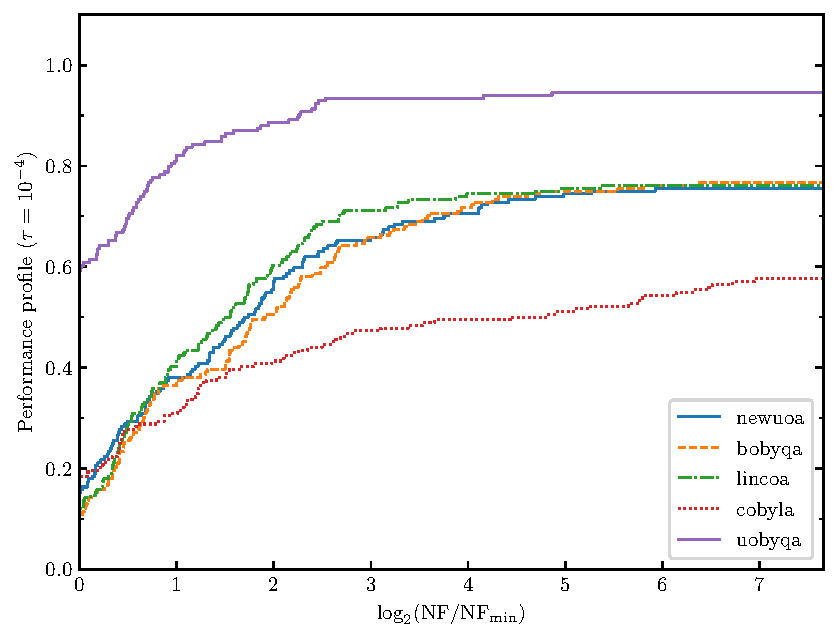
\includegraphics[width=\textwidth]{pp10.pdf}
        \caption{Dimension at most~$10$.}
        \label{fig:ppu-10}
    \end{subfigure}
    \hfill
    \begin{subfigure}{.48\textwidth}
        \centering
        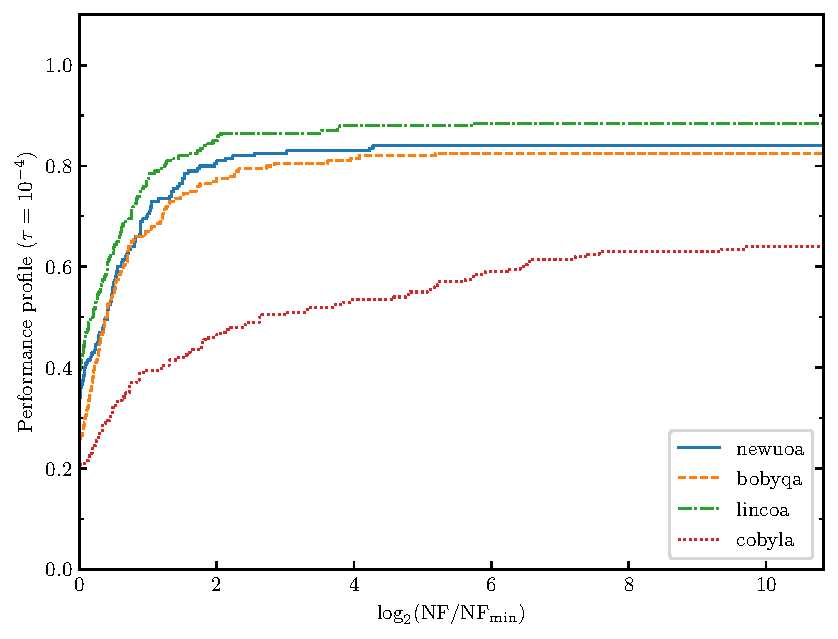
\includegraphics[width=\textwidth]{pp50.pdf}
        \caption{Dimension at most~$10$.}
        \label{fig:ppu-50}
    \end{subfigure}
    \caption{Performance profile on unconstrained problems with a precision~$\tau = 10^{-4}$.}
        % \label{fig:ppu}
\end{figure}

Consider however the following experiment.
Given a smooth objective function~$\obj$, assume that the value received by the solvers is
$$F_{\sigma}(x) = [1 + \sigma e(x)] \obj(x),$$
where~$e(x)$ is a random variable that follows a standard normal distribution~$\mathcal{N}(0, 1)$, and~$\sigma \ge 0$ is a given noise level.
\Cref{fig:ppun-50} presents the performance profiles on the same unconstrained problems of dimension at most~$50$ from the CUTEst library as the previous experiment by randomizing the objective functions as~$F_{\sigma}$ with~$\sigma = 10^{-2}$.
Because of the stochastic behavior of the experiment, the convergence test~\cref{eq:cvt} needs to be adapted.
Each problem is solved~$10$ times by each solver, the objective value considered at each iteration is the average value for all runs, and the optimal value~$f_{\ast}$ of a given problem is decided as follows.
It is the least value reached by the solvers for every run on the noised variation of the problem and by all the solvers on the noise-free original problem.
In doing so, one should expect a decrease of the proportion of problems solved when compared with the previous experiment.

\begin{figure}[ht]
    \centering
    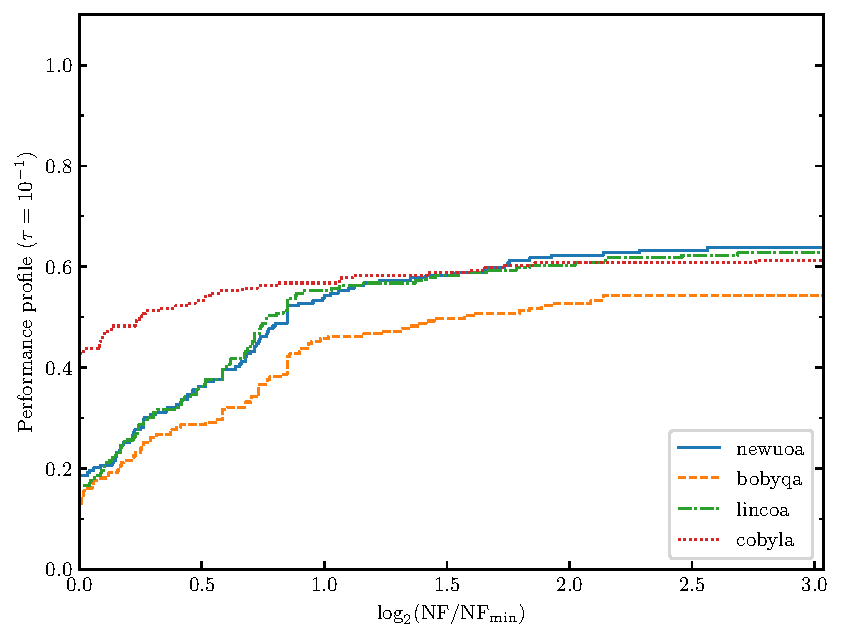
\includegraphics[width=.48\textwidth]{pp50-noisy.pdf}
    \caption{Performance profile on noised variations of unconstrained problems of dimension at most~$50$ with a precision~$\tau = 10^{-1}$.}
    \label{fig:ppun-50}
\end{figure}

We observe however a peculiar behavior of \gls{cobyla} on this experiment, as it defeats all other solvers on unconstrained problems even though it is not defined for such kind of problem, and uses the simplest models.
It seems that the linear models of \gls{cobyla} are, in some sense, less sensitive to Gaussian noise, but the authors did not derive a theory for this behavior as of today.

\subsubsection{An example of hyperparameter tuning problem}

We consider now the more practical problem of the hyperparameter tuning of a \gls{svm}.
The model we consider is a~$C$-SVM~\cite{Chang_Lin_2011} for binary classification problems with an \gls{rbf} kernel, admitting two hyperparameters: a regularization parameter~$C > 0$ and a kernel parameter~$\gamma > 0$.
We want to compare the performance of PDFO with a prominent Bayesian optimization method and \gls{rs}.
To this end, we use the \python\ package \texttt{hyperopt}~\cite{Bergstra_Yamins_Cox_2013} for solving the optimization problems, which provides both \gls{tpe} and \gls{rs} methods.
Our experiments are based on binary classifications problems from the \libsvm\ datasets\footnote{Available at \url{https://www.csie.ntu.edu.tw/~cjlin/libsvmtools/datasets/}.}.
A description of the datasets employed is provided in \cref{tab:htdata}.

\begin{table}[ht]
    \caption{Considered \libsvm\ datasets description}
    \label{tab:htdata}
    \centering
    \begin{tabular}{ccS[table-parse-only]S[table-parse-only]}
        \toprule
        Dataset~$\mathcal{P}$   & Attribute characteristic  & {Dimension~$d$}   & {Dataset size}\\
        \midrule
        splice                  & $[-1, 1]$, scaled         & 60                & 1000\\
        svmguide1               & $[-1, 1]$, scaled         & 4                 & 3088\\
        svmguide3               & $[-1, 1]$, scaled         & 21                & 1242\\
        ijcnn1                  & $[-1, 1]$                 & 22                & 49990\\
        \bottomrule
    \end{tabular}
\end{table}

The problem we consider is as follows.
A dataset~$\mathcal{P} \subseteq [-1, 1]^d$ from \cref{tab:htdata} is randomly split into a training dataset~$\mathcal{L}$, admitting approximately~$70\%$ of the data, and a testing dataset~$\mathcal{T}$, with~$\mathcal{P} = \mathcal{L} \cup \mathcal{T}$.
We want to maximize the~$5$-fold \gls{auc} validation score of the \gls{svm} trained on~$\mathcal{L}$ with respect to the hyperparameters~$C$ and~$\gamma$.
The \gls{auc} score, a real number in~$[0, 1]$, measures the area underneath the \gls{roc} curve, a graph representing the performance of a binary classification model.
This curve plots the true positive classification rate with respect to the false positive classification rate at different classification thresholds.
The~$5$-fold \gls{auc} validation score corresponds to the following.
The set~$\mathcal{L}$ is split into~$5$ folds, and the model is trained~$5$ times, on each union of~$4$ distinct folds.
After each training, the \gls{auc} score is calculated on the last fold, which was not involved in the training process, giving rise to~$5$ \gls{auc} scores, the average of which corresponds to the~$5$-fold \gls{auc} validation score.
It is then clear that such an experiment lies in the \gls{dfo} context.

The numerical results for this experiment are provided in \cref{sec:htres}.
The \gls{auc} scores and accuracies presented in the tables correspond to the ones computed on~$\mathcal{T}$ with an \gls{svm} trained on~$\mathcal{L}$, with the tuned parameters~$C$ and~$\gamma$.
In a nutshell, it globally shows that the numerical performances of \gls{pdfo} against the two classical approaches are very similar, but the computations requires much fewer \gls{auc} evaluations, and hence, much less computation time.
This behavior is particularly visible on the dataset \enquote{ijcnn1} in \cref{tab:ijcnn1}, as the size of this dataset is much larger than the others.
Thus, we can conclude that \gls{pdfo} performed better than the package \texttt{hyperopt} on these problems, even though the final numerical results are mostly similar.

\section{Conclusions}

We have presented the package \gls{pdfo} for \matlab\ and \python, which aims at simplifying the use of the Powell's \gls{dfo} solvers.
A more complete presentation of the package itself can be found on the \gls{pdfo} website, together with different examples of use.
The scope of \gls{pdfo} in the future is not limited only to the Powell's \gls{dfo} solvers.
The authors are currently working on a new solver for nonlinearly-constrained optimization, which is aimed to be added to \gls{pdfo}, and other \gls{dfo} solvers may be included in the future to \gls{pdfo}.

\printbibliography

\appendix
\clearpage

\section{Hyperparameter tuning experiment results}
\label{sec:htres}

\begin{table}[!ht]
    \caption{Hyperparameter tuning problem on the dataset \enquote{splice}.}
    % \label{tab:splice}
    \centering
    \begin{tabular}{cS[table-parse-only]SSS}
        \toprule
        Solver                          &
            {No.\ eval.}                &
            {AUC Score ($10^{-1}$)}     &
            {Accuracy ($10^{-1}$)}      &
            {Execution time (\si{\second})}\\
        \midrule
        \gls{pdfo}  & 65    & 9.568 & 9.933 & 3.697\\
        \gls{rs}    & 100   & 6.409 & 5.300 & 4.635\\
        \gls{rs}    & 200   & 7.880 & 5.300 & 9.244\\
        \gls{rs}    & 300   & 7.880 & 5.300 & 13.763\\
        \gls{tpe}   & 100   & 5.000 & 5.033 & 4.889\\
        \gls{tpe}   & 300   & 7.736 & 5.300 & 15.726\\
        \bottomrule
    \end{tabular}
\end{table}

\begin{table}[!ht]
    \caption{Hyperparameter tuning problem on the dataset \enquote{svmguide1}.}
    % \label{tab:svmguide1}
    \centering
    \begin{tabular}{cS[table-parse-only]SSS}
        \toprule
        Solver                          &
            {No.\ eval.}                &
            {AUC Score ($10^{-1}$)}     &
            {Accuracy ($10^{-1}$)}      &
            {Execution time (\si{\second})}\\
        \midrule
        \gls{pdfo}  & 68    & 9.966 & 9.730 & 4.906\\
        \gls{rs}    & 100   & 9.966 & 9.676 & 16.178\\
        \gls{rs}    & 200   & 9.966 & 9.676 & 32.914\\
        \gls{rs}    & 300   & 9.966 & 9.676 & 48.404\\
        \gls{tpe}   & 100   & 9.966 & 9.720 & 13.057\\
        \gls{tpe}   & 300   & 9.966 & 9.720 & 33.392\\
        \bottomrule
    \end{tabular}
\end{table}

\begin{table}[!ht]
    \caption{Hyperparameter tuning problem on the dataset \enquote{svmguide3}.}
    % \label{tab:svmguide3}
    \centering
    \begin{tabular}{cS[table-parse-only]SSS}
        \toprule
        Solver                          &
            {No.\ eval.}                &
            {AUC Score ($10^{-1}$)}     &
            {Accuracy ($10^{-1}$)}      &
            {Execution time (\si{\second})}\\
        \midrule
        \gls{pdfo}  & 68    & 8.241 & 8.016 & 2.793\\
        \gls{rs}    & 100   & 8.025 & 7.882 & 4.233\\
        \gls{rs}    & 200   & 8.141 & 7.775 & 8.308\\
        \gls{rs}    & 300   & 8.141 & 7.775 & 12.414\\
        \gls{tpe}   & 100   & 7.774 & 7.453 & 4.197\\
        \gls{tpe}   & 300   & 8.106 & 7.989 & 12.912\\
        \bottomrule
    \end{tabular}
\end{table}

\begin{table}[!ht]
    \caption{Hyperparameter tuning problem on the dataset \enquote{ijcnn1}.}
    \label{tab:ijcnn1}
    \centering
    \begin{tabular}{cS[table-parse-only]SSS}
        \toprule
        Solver                          &
            {No.\ eval.}                &
            {AUC Score ($10^{-1}$)}     &
            {Accuracy ($10^{-1}$)}      &
            {Execution time (\SI{}[10^3]{\second})}\\
        \midrule
        \gls{pdfo}  & 59    & 9.940 & 9.819 & 1.892\\
        \gls{rs}    & 100   & 9.886 & 9.773 & 4.435\\
        \gls{rs}    & 200   & 9.886 & 9.773 & 9.146\\
        \gls{rs}    & 300   & 9.886 & 9.773 & 13.251\\
        \gls{tpe}   & 100   & 9.891 & 9.791 & 4.426\\
        \gls{tpe}   & 300   & 9.896 & 9.786 & 12.552\\
        \bottomrule
    \end{tabular}
\end{table}

\section{Fake section}
\label{sec:fake}

\end{document}
